\begin{titlepage}
    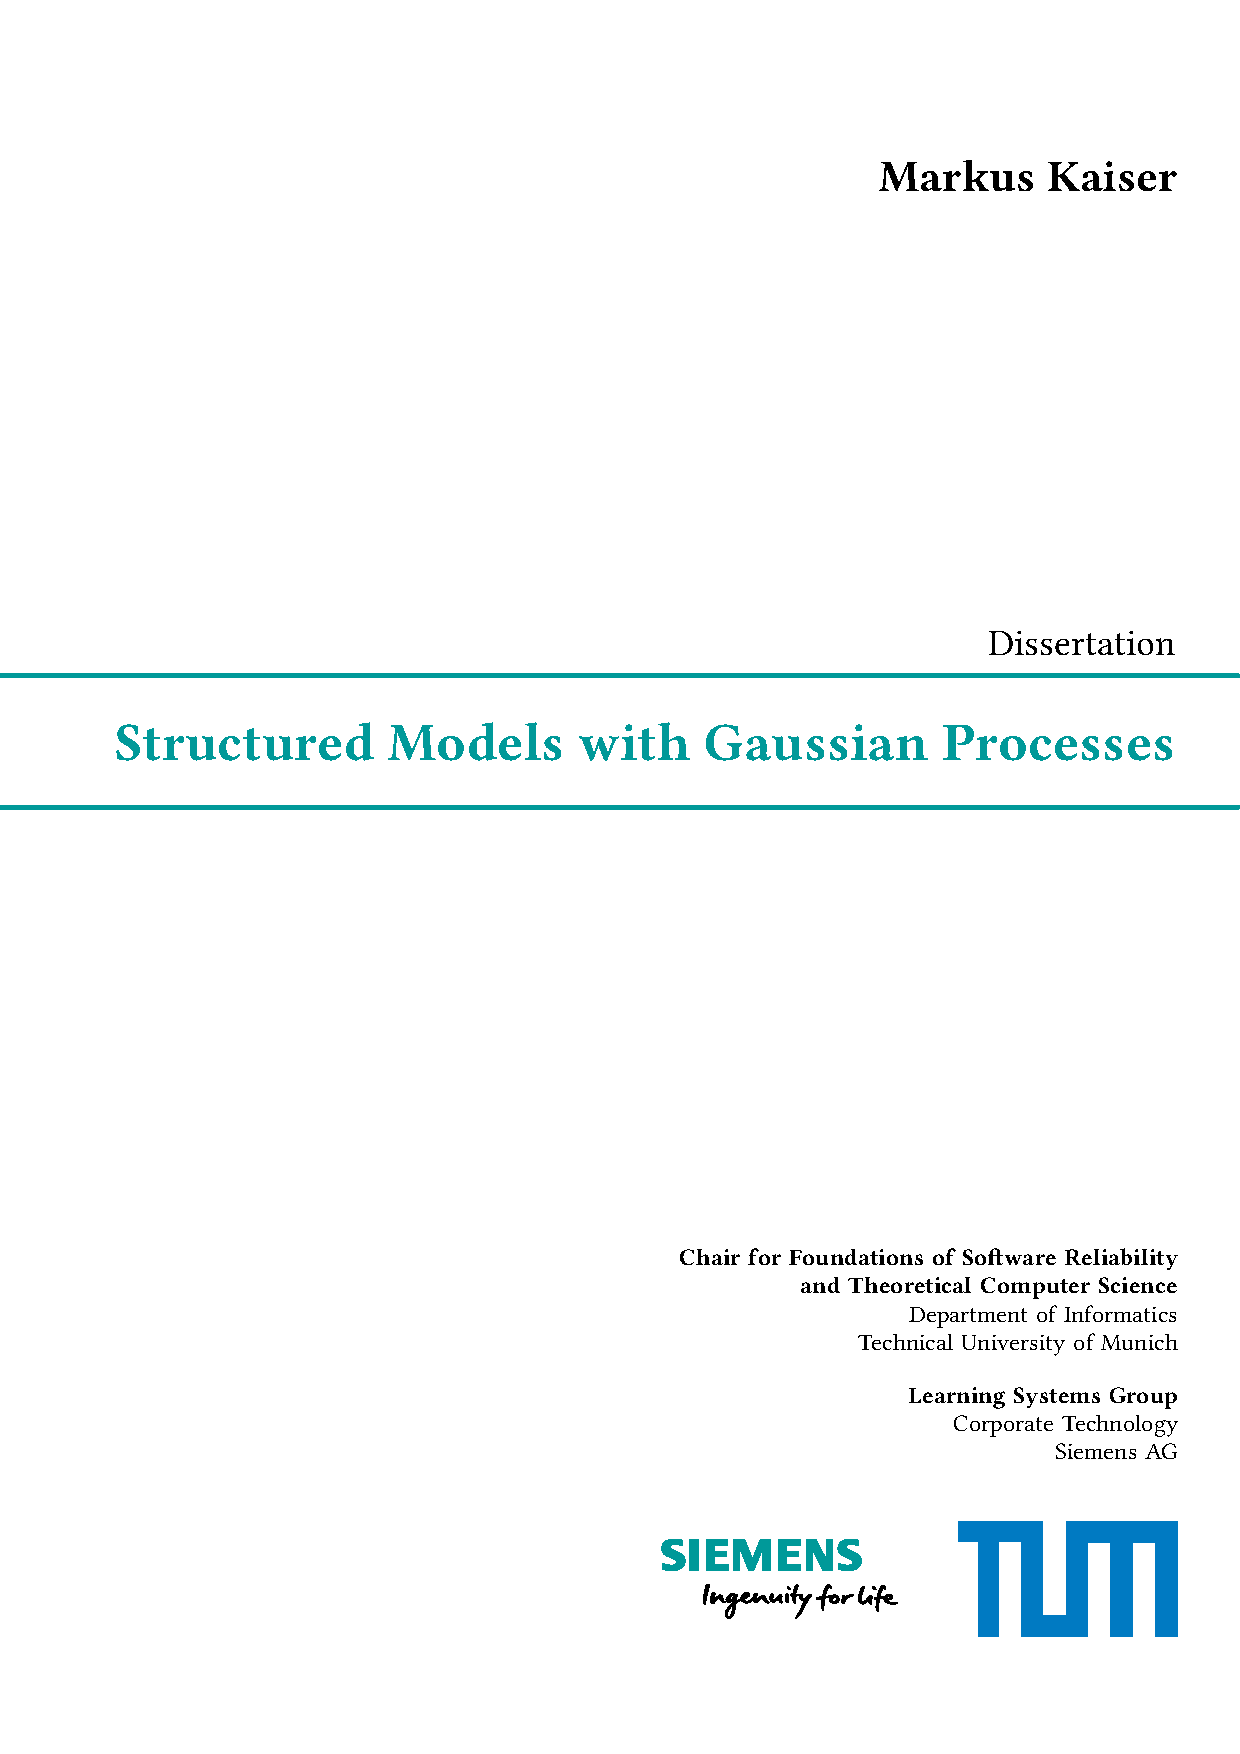
\includepdf{figures/title_page}
\end{titlepage}

\begin{titlepage}
    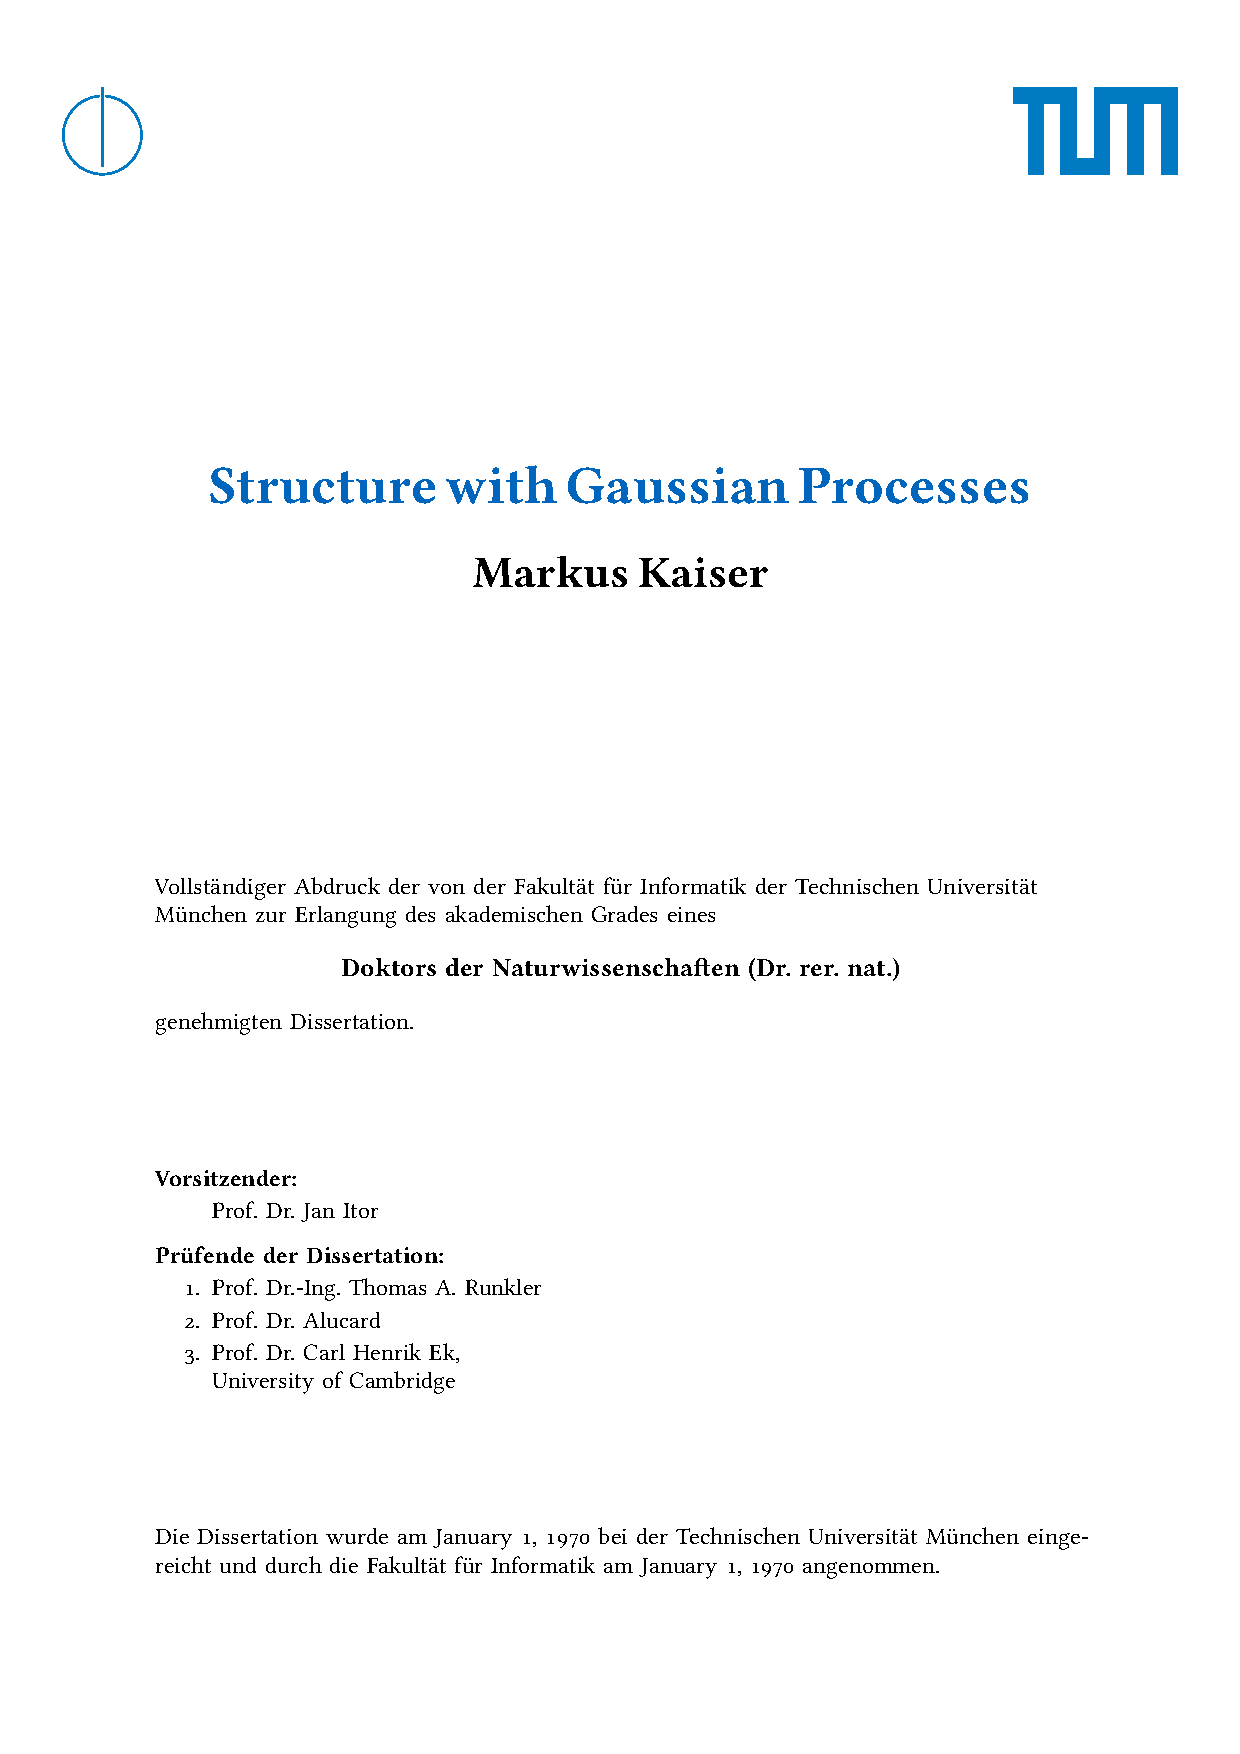
\includepdf{figures/title_page_tum}
\end{titlepage}

\begin{Abstract}{ngerman}
    Mit Methoden des maschinellen Lernens konnten in den letzten Jahren in einer Vielzahl von digitalen Anwendungsbereichen wie Spracherkennung, Computer-Vision oder Videospielen beeindruckende Erfolge erzielt werden.
    Der Transfer zu Anwendungen in der physikalischen Welt hat sich jedoch als eine Herausforderung erwiesen, da sie eine Reihe neuer Anforderungen mit sich bringen.
    Lernverfahren müssen Expertenwissen effizient nutzen, mit wenigen Daten auskommen und Unsicherheiten bestimmen.
    In dieser Dissertation wird untersucht, wie strukturierte probabilistische Modelle es uns ermöglichen, diesen Anforderungen gerecht zu werden.
    Strukturierte Modelle kombinieren datengestützte und theoriegetriebene Modellierungsansätze, um Expertenwissen zu formalisieren und dennoch neue Erkenntnisse aus Daten gewinnen zu können.

    In dieser Arbeit werden probabilistische strukturierte Modelle mithilfe von bayesschen nicht-parametrischen Methoden formuliert.
    Wir nutzen Informationen über die Struktur eines Lernproblems, um Modelle zu formulieren, die Wissen reproduzieren, für Domänenexperten verständlich sind, physikalisch plausible Vorhersagen in unbekannten Situationen liefern und ihre eigene Unsicherheit beziffern können.
    Dazu bettwen wir allgemeine Funktionsapproximatoren in probabilistische Modelle ein und formulieren Inferenzmethoden auf Basis von verketteten und hierarchischen Gaußprozessen.
    Am Beispiel realer industrieller Anwendungen wie der Erkennung fehlerhafter Sensoren und der der Vorhersage der Stromerzeugung in einem Windpark zeigen wir, dass strukturierte informative Unsicherheiten liefern, interpretierbar sind und erfolgreich generalisieren.

    In Situationen in denen die interne Struktur oder das Generalisierungsverhalten von Modellen in den Mittelpunkt rücken kann Modellselektion basierend auf klassischen Metriken unzureichend sein, um bevorzugte Modelle zu identifizieren.
    Wir formalisieren den subjektiven Anteil der Modellselektion, indem wir die Aufgabe, die ein Modell lösen soll, in die Auswahl mit einbeziehen.
    Wir zeigen an einem Reinforcement-Learning Problem, dass semantisch korrekte Modelle andere Modelle mit ähnlichen Metriken übertreffen und es Experten ermöglichen, das Verhalten von Agenten zu beeinflussen.
    Wir untersuchen die Eigenschaften strukturierter Modelle in einem breiteren Kontext und diskutieren die Grenzen gängiger Inferenzverfahren, warum Modelle mit suboptimalen Metriken in hierarchischen Systemen erfolgreich eingesetzt werden können und wie bayessche Inferenzprobleme formulierten werden können, die nachgelagerte Aufgaben berücksichtigen.
\end{Abstract}

\begin{Abstract}{english}
    Machine learning methods have seen great success recently in a wide range of digital domains such as speech recognition, computer vision or video games.
    However, bridging the gap to applications in the physical world has proved challenging as they introduce a new set of requirements.
    Machine learning systems must make efficient use of expert knowledge, handle low data regimes, and quantify uncertainties.
    This thesis explores how structured probabilistic models allow us to cope with these requirements.
    Structured models combine black-box and white-box modeling approaches to formalize expert knowledge while still being able to gain new insights from data.

    In this work, we formulate Bayesian structured models using methods from Bayesian nonparametrics.
    We use information about the structure of a learning problem to formulate machine learning models that reproduce knowledge, are understandable for domain-experts, make physically plausible predictions in unseen situations and can quantify their own uncertainty.
    We explore how to embed general function approximators in Bayesian probabilistic models to enforce structure and discuss how to formulate inference schemes based on composite and hierarchical Gaussian process models.
    Using real-world industrial applications such as the detection of faulty sensors and the prediction of power generation in a wind-farm as examples, we show how to use structured models to factorize uncertainties, achieve interpretability, and generalize to unobserved inputs.

    In settings where internal structure and generalization behavior come into focus, model selection using marginal likelihoods can be insufficient to identify desirable models.
    We consider how to formalize the subjectiveness in model selection through the task a model will be used to solve.
    We show that in a reinforcement learning problem, semantic models outperform other models with similar performance metrics and allow experts to influence agent behavior.
    We explore the properties of structured models in a broader context and discuss the limits of current inference schemes, why models with suboptimal marginal likelihoods can perform well in hierarchical systems, and how to formulate Bayesian inference problems that take downstream tasks into account.
\end{Abstract}

\begin{Acknowledgements}
    I want to thank my supervisor Prof.~Dr.~Thomas A.~Runkler for his guidance and support.
    Thomas has always encouraged me to explore my ideas while offering invaluable advice and making sure I do not lose focus.
    I am very grateful to my co-supervisor Prof.~Dr.~Carl Henrik Ek for his enthusiasm and mentorship.
    He is an inspiring teacher and shows me what is important in academia.
    Thank you for welcoming me to your research group, making Bristol a second home for me, and the countless discussions about the big picture and the small details.
    I also want to thank my advisor Dr.~Clemens Otte for his valuable input and his exceptional ability to combine research and applications.
    I could not have asked for better supervision or a more encouraging research environment during my studies.

    I am thankful to everyone at Siemens and the Learning Systems group, especially Volkmar Sterzing for giving us PhD candidates the freedom to pursue our interests and enabling us to work on exciting industrial applications.
    I am grateful to Steffen Udluft and Hans Georg Zimmermann for always taking the time to discuss new ideas and for broadening my horizon as well as my fellow PhD candidates Stefan Depeweg, Daniel Hein and Phillip Swazinna for many discussions, whiteboard-drawings and meetings at the Biergarten.
    Thanks to Marion Eigner for her refreshing perspective and friendship.

    I feel lucky to be part of a motivating and unique group in Bristol and Bath.
    Thank you to Prof.~Dr.~Neill Campbell for your passion for good research and for your help in pursuing worthwhile ideas.
    I want to thank Erik Bodin, Ieva Kazlauskaite and Ivan Ustyuzhaniov for many thoughtful discussions and collaborations.

    A big thank you to my siblings Matthias and Andrea for your support and encouragement.
    I sincerely thank my parents, Pia and Robert Kaiser, for enabling and inspiring us to follow our dreams and for your unconditional support.
    Above all I want to thank Hannah for her patience and understanding while being in COVID-19 lockdown with somebody writing their thesis.
    Thank you for all the lunches, the much-needed distractions, the happiness, and your love.
\end{Acknowledgements}

\listoftodos
\todototoc

\tableofcontents
